\section{Funcionamiento general}

\begin{frame}
    \begin{columns}[t]
        \begin{column}{.5\textwidth}
          \tableofcontents[sections={1-2},currentsection]
        \end{column}
        \begin{column}{.5\textwidth}
          \tableofcontents[sections={3-4},currentsection]
        \end{column}
    \end{columns}
\end{frame}

\subsection{Bases del funcionamiento}
\begin{frame}[fragile]{}

Moogle! se basa principalmente en:
\begin{itemize}
\item Modelo Vectorial
\item Tf-Idf
\item Similitud Coseno

\end{itemize}

\pause
\vspace{5mm}
¿Pero, en qué consiste cada uno?

\end{frame}

\subsection{Modelo Vectorial}
\begin{frame}[fragile]{Modelo Vectorial}

El modelo vectorial se basa expresar cada
documento como vectores de la misma dimension usando la relevancia de cada palabra
\pause

\begin{figure}[h]
    \center
    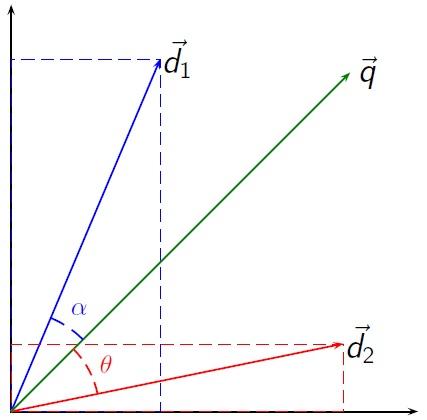
\includegraphics[width=4cm]{Vectormodel.jpg}
    \caption{Modelo Vectorial}
\end{figure}

\end{frame}

\subsection{Tf-Idf}
\begin{frame}[fragile]{Tf-Idf}

Term frecuency – Inverse term frecuency, es un valor que se utiliza para calcular la relevancia de cada palabra.


\pause
$ tf(t,d) $: cantidad de veces que aparece el término $t$ en el documento $d$ del conjunto de documentos $D$ 
%aqui va la formulita
\begin{equation}
    idf(t,D) = \log{\frac{|D|}{|\{d\in{D}:t\in{d}\}|}}
\end{equation}
\begin{equation}
    tfidf(t,d,D) = tf(t,d)*idf(t,D)
\end{equation}


\end{frame}

\subsection{Similitud Coseno}
\begin{frame}{Similitud Coseno}

La similitud consiste en calcular la relevancia entre dos de los vectores (documentos) a partir del valor del coseno del ángulo comprendido
\pause

\begin{figure}[h]
    \center
    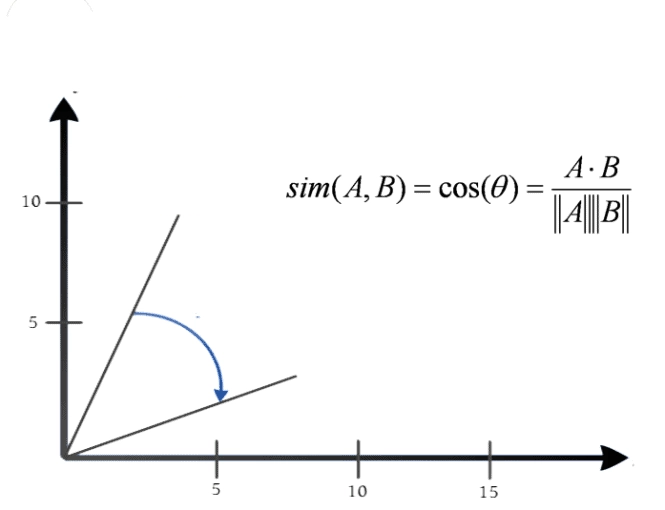
\includegraphics[width=6cm]{cosinesimilarity.png}
    \caption{Similitud Coseno}
\end{figure}

\end{frame}


